\chapter{Introduction}

\section{Overview of Neutrino Physics}

On December 4 1930, in an open letter addressed to "Dear Radioactive Ladies and Gentlemen" attempting to salvage one of the most fundamental principles in physics, energy conservation, W. Pauli postulated a neutral weakly interacting particle which is later dubbed \emph{neutrino} and opened up neutrino physics. In 1934, E. Fermi formulated the first successful theory of weak interactions, the Fermi theory of $\beta$-decay.

\section{Neutrino Oscillation and \texorpdfstring{$\theta_{13}$}{theta13}}

\subsection{Neutrino Mixing and Neutrino Oscillation}
According to the Standard Model of Particle Physics, there are 3 flavors of neutrinos, namely, $\nu_e$, $\nu_\mu$ and $\nu_\tau$. These are the eigenstates when neutrinos take part in weak interactions. However, these are not the eigenstates when neutrinos propagate freely in space. Since neutrinos have minute but nonzero mass, there are 3 mass eigenstates and the relation between flavor and mass eigenstates can be written as
\begin{equation}
\left( \begin{array}{c} \nu_e \\ \nu_\mu \\ \nu_\tau \end{array} \right)
=
\begin{pmatrix}
U_{e1} & U_{e2} & U_{e3} \\
U_{\mu1} & U_{\mu2} & U_{\mu3} \\
U_{\tau1} & U_{\tau2} & U_{\tau3}
\end{pmatrix}
\left( \begin{array}{c} \nu_1 \\ \nu_2 \\ \nu_3 \end{array} \right)
\end{equation}

The unitary matrix $[U_{lj}]$ is called PMNS matrix named after physicists B. Pontecorvo, Z. Maki, M. Nakagawa, and S. Sakata and can be parametrized by

\allowdisplaybreaks
\begin{align}
U_{PMNS}=
\begin{pmatrix}
c_{12}c_{13} & s_{12}c_{13} & s_{13}e^{-i\delta} \\
-s_{12}c_{23}-c_{12}s_{23}s_{13}e^{-i\delta} & c_{12}c_{23}-s_{12}s_{23}s_{13}e^{-i\delta} & s_{23}c_{13} \\
s_{12}s_{23}-c_{12}c_{23}s_{13}e^{-i\delta} & -c_{12}s_{23}-s_{12}c_{23}s_{13}e^{-i\delta} & c_{23}c_{13}
\end{pmatrix}
\begin{pmatrix}
e^{i\phi_1} & 0 & 0 \\
0 & e^{i\phi_2} & 0 \\
0 & 0 & 1
\end{pmatrix}
\end{align}

If an electron antineutrino $\bar{\nu}_e$ is produced at the source and propagates in space, at a distance $L$ away from the source the survival probability, i.e. the probability that the neutrino doesn't change to other flavors, is
\allowdisplaybreaks
\begin{align}
P(\bar{\nu}_e\rightarrow\bar{\nu}_e)=1-c^4_{13}\sin^22\theta_{12}\sin^2\Delta_{21}-c^2_{12}\sin^22\theta_{13}\sin^2\Delta_{31}-s^2_{12}\sin^22\theta_{13}\sin^2\Delta_{32}
\end{align}

Among the three mixing angles $\theta_{13}$ was the only unknown parameter, and the goal of Daya Bay experiment was to measure $\sin^22\theta_{13}$ with $0.01$ sensitivity at $90\%$ confidence level.


\subsection{Neutrino Flux and Energy Spectrum}

Nuclear power is generated by fission reactions mainly from 4 kinds of isotopes, namely $^{235}$U, $^{239}$Pu, $^{238}$U and $^{241}$Pu. The fission products then undergo beta decay and generate neutrinos. Each fission reaction on average produces about 6 neutrinos. The detailed neutrino flux and energy spectrum at a particular time depend on the composition of the isotopes, the total reactor thermal power, the fission rate of individual isotopes and the spectrum of the individual isotopes. The number of neutrinos released by the reactor per unit time is
\begin{equation} \label{eq:neutrino_flux}
  \phi(E)=\frac{W_{th}}{\sum\limits_{i=1}^4f_ie_i}\sum\limits_{i=1}^4f_iS_i(E)
\end{equation}
where $i$ runs over the four main isotopes, $W_{th}$ is the total thermal power, $f_i$ is the fission fraction, $e_i$ is the fission energy release and $S_i(E)$ is the neutrino energy spectrum.

The fission fraction of each isotope and the total thermal power are monitored and the weekly averaged numbers are offered by the nuclear power plant. $e_i$ is the part of the fission energy that converts into heat. Typical values at the midpoint of the reactor operation period is given in Table~\ref{table:thermal_fission_energy}~\cite{Kopeikin2004}.
\begin{table}
	\centering
	\begin{tabular}{|c|c|}
	\hline
	isotope & $e_i$ (MeV/fission) \\
	\hline
	$^{235}$U & 201.92 ± 0.46 \\
	$^{238}$U & 205.52 ± 0.96 \\
	$^{239}$Pu & 209.99 ± 0.60 \\
	$^{241}$Pu & 213.60 ± 0.65 \\
	\hline
	\end{tabular}
	\caption{Typical thermal fission energy $e_i$ at the midpoint of the reactor operation period.}
	\label{table:thermal_fission_energy}
\end{table}

The antineutrino spectra $S_i(E)$ can be calculated theoretically. A three parameter calculation was done by Vogel and Engel~\cite{Vogel1989}. Figure~\ref{figure:isotope_antineutrino_spectra} shows the spectra of the four dominant isotopes. $^{238}$U produces the most antineutrinos per fission while $^{239}$Pu produces the least.
\begin{figure}
	\centering
	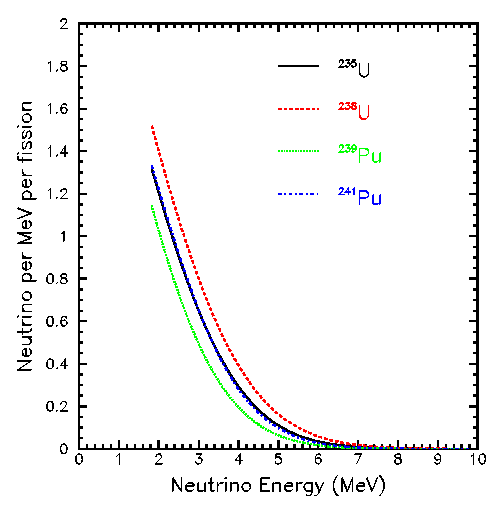
\includegraphics[width=.5\textwidth]{figures/chap1/isotope_antineutrino_spectra.eps}
	\caption{Calculated antineutrinos spectra for each dominant isotope.}
	\label{figure:isotope_antineutrino_spectra}
\end{figure}


\subsection{\texorpdfstring{$\bar{\nu}_e$}{Electron Antineutrino} Detection}
Daya Bay utilizes the renowned Cowan–Reines method of prompt-delayed coincidence to detect $\bar{\nu}_e$. The reaction involved in this method is the inverse beta decay (IBD),
\begin{equation}
	\bar{\nu}_e+p\longrightarrow e^++n
\end{equation}
The positron is quickly annihilated by an electron and releases photons which constitute the prompt signal. The neutron propagates in the target medium, slows down mainly by collisions with protons and finally gets captured by some nucleus which in turn de-excites and releases photons constituting the delayed signal. Such prompt-delayed coincidence forms a very definitive $\bar{\nu}_e$ signature and greatly suppresses backgrounds.

The antineutrino event rate is given by
\begin{equation}
	R=\int \epsilon(E)P_{\bar{\nu}_e\rightarrow\bar{\nu}_e}(L,E)\frac{N_p\sigma(E)}{4\pi L^2}\phi(E)dE
\end{equation}
where $\epsilon$ is the antineutrino detection efficiency, $P_{\bar{\nu}_e\rightarrow\bar{\nu}_e}$ is the antineutrino survival probability, $N_p$ is the number of protons in the detector, $\sigma$ is the IBD total cross section, $L$ is the distance from the reactor core to the detector and $\phi$ is the number of released antineutrinos per unit time given in Eq.~\ref{eq:neutrino_flux}.

$P_{\bar{\nu}_e\rightarrow\bar{\nu}_e}$ depends on $\sin^22\theta_{13}$ which we want to infer from the measured IBD rates. $\epsilon$, $N_p$ and $L$ are measured by auxiliary methods and instruments which will be detailed later. The total cross section of the IBD reaction in the limit of infinite nucleon mass can be written as~\cite{Vogel1999}
\begin{equation}
	\sigma^{(0)}_{tot}=0.0952\times 10^{-42} \left( \frac{E^{(0)}_ep^{(0)}_e}{1 MeV^2}\right) cm^2
\end{equation}
where $E^{(0)}_e$ and $p^{(0)}_e$ are the energy and momentum of the positron, respectively. The next-to-leading order term in $1/M$, the inverse nucleon mass, is nonnegligible. The total cross section to first order in $1/M$ is shown in Figure~\ref{fig:IBD_total_cross_section} and is adopted in Daya Bay's $\theta_{13}$ analysis.
\begin{figure}
	\centering
	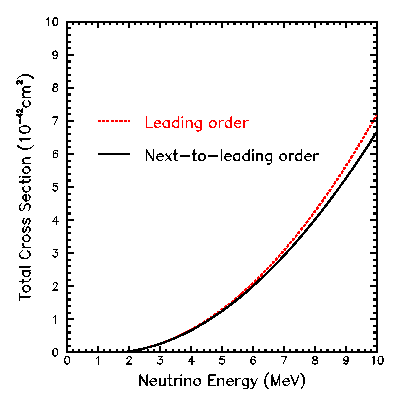
\includegraphics[width=.4\textwidth]{figures/chap1/IBD_total_cross_section.eps}
	\caption{The IBD total cross section calculated to the leading order and next-to-leading order terms.}
	\label{fig:IBD_total_cross_section}
\end{figure}

\section{Muon Induced Backgrounds}

The Earth is constantly bombarded by high energy particles known as cosmic rays. The primary source of cosmic ray is protons. When protons interact with the air molecules, secondary particles originate which in turn decay and generate muons, neutrinos, electrons and photons. Figure~\ref{figure:atmospheric_cosmic_rays} shows the vertical fluxes of the dominant cosmic ray components estimated from the intensity of primary nucleons incident on top of the atmosphere. At sea level (altitude = 0) there are still high fluxes of cosmic rays ranging from about 0.1 to 100 $m^{-2}s^{-1}sr^{-1}$. Fortunately rocks are very good natural shielding from the particles and when one goes deep enough underground only muons and neutrinos can survive. Therefore sensitive experiments go underground and the main sources of background would be the natural radioactivity from rocks as well as muons and particles or isotopes induced by muons.
\begin{figure}
	\centering
	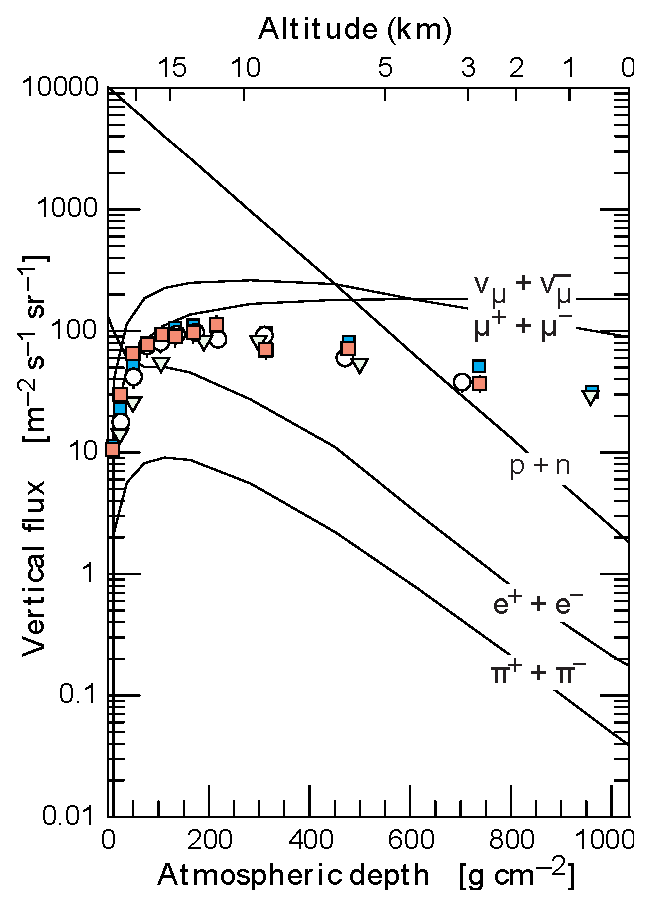
\includegraphics[width=.5\textwidth]{figures/chap1/atmospheric_cosmic_rays.eps}
	\caption{Estimated vertical fluxes of major cosmic ray components. Points are measurements of negative muons with energy larger than 1 GeV.}
	\label{figure:atmospheric_cosmic_rays}
\end{figure}

Daya Bay's experimental halls are also underground, and the muon induced neutrons and isotopes constitute one of the major background sources. For Daya Bay, the sea level muon energy and angular distribution is important because in order to get the energy and angular distribution in each hall with Monte Carlo simulation, the sea level data together with the mountain overburden profile and the rock composition is input into the simulation and the muons are then propagated through the rock to get the propagated energy and angular distribution for those survived to the ceiling of the halls. Conventionally the sea level muon flux is described by the Geisser's formula~\cite{Beringer2012},
\begin{equation}
\frac{dN_\mu}{dE_\mu d\Omega}=\frac{0.14E_\mu^{-2.7}}{cm^2\cdot s \cdot sr \cdot GeV}\left\lbrace \frac{1}{1+\frac{1.1E_\mu\cos\theta}{115GeV}}+\frac{0.054}{1+\frac{1.1E_\mu\cos\theta}{850GeV}} \right\rbrace
\end{equation}
where the two terms in the braces give the contribution of pions and kaons, respectively.